\chapter{绪论}\label{capater:intro}
轨迹大数据是移动物联网时代的产物,记录了移动对象的行为信息。通过轨迹数据分析技术可以挖掘人类活动规律与行为特征、城市车辆的移动模式、大气环境变化规律等信息。这些挖掘成果为研究城市发展、社会变迁和自然环境演变提供重要的参考价值。本文重点研究了分布式$k$近邻轨迹查询问题。本章中,章节~\ref{sec-c1-background}阐述了分布式轨迹数据相似性查询的研究现状;章节~\ref{sec-c1-content}详述了本文的具体研究内容以及所遇到的挑战;章节~\ref{sec-c1-contribution}简述了本文的主要研究方法和研究贡献。

\section{研究背景}\label{sec-c1-background}
        随着卫星定位导航、无线通信和普适计算等高新技术的不断发展,带有定位功能的移动智能设备已被广泛应用,并成为社会生产、生活的重要组成部分。移动对象(含人、动物和车辆等)在主动或被动使用这些设备的同时,产生了大量记录其移动历史行为的轨迹数据(Trajectory Data)。例如:滴滴出行,全球最大的一站式多元化出行平台,在2017年10月发布的《第三季度全国重点城市交通出行报告》中称其每天新增的定位轨迹数据超过70TB\footnote{http://www.xiaojukeji.com/index/index}。
            轨迹数据是地理空间在时间轴上形成的多维空间中的一条曲线,表示了移动对象在一段时间内时空信息等移动行为的变化。每条轨迹可看作一条时空采样点构成的序列,其中每个采样点记录了时间、位置、速度、方向等信息。 从微观角度将,轨迹数据蕴含了移动对象的移动模式与规律\cite{Gonz2008Understanding,Song2010Limits,LiDHKN10},例如从轨迹数据种我们可以发现市民的居住地、工作地和消费娱乐场所\cite{zzgSF}。从宏观角度来讲,海量的轨迹大数据蕴含了群体的移动迁徙和社会发展的变化,如城市的发展、交通的演化以及社会的变迁\cite{Zheng15}。通过轨迹分析等手段进行知识发现,并将它们运用在各种交通和服务应用系统中,包括交通导航\cite{QSJPredict,QSJProjection}、交通智能指挥\cite{LXX}、车辆异常监控\cite{CJY,MJLSoftware}、物流配送、城市规划、军事调度等\cite{QGD,XJJZXF,GQSurvery}。
        
         海量的轨迹数据具有重要的社会和应用价值,不仅为解决拥堵、改善交通服务、缓解能源紧缺和降低大气污染等社会问题提供了新的机遇,而且对认知人民的社会活动、优化公共资源配置、为建立新型共享经济有着特殊的意义。2017年12月8日,习近平总书记在中共中央政治局第二次集体学习时强调:实施国家大数据战略,加快建设数字中国。因此,轨迹大数据称为政府和企业的重要资源财富并得到广泛重视。
         在此背景下,轨迹大数据的分析和挖掘已经被学术界和工业界大量研究并成为数据挖掘领域的重要的新兴分支。在工业界,百度地图能根据实时轨迹数据进行路径规划。摩拜进行了基于自行车骑行目的地预测的研究\footnote{https://www.biendata.com/competition/mobike/}。美团和饿了么等外卖公司设计了基于轨迹数据的智能派单系统\footnote{http://blog.csdn.net/jinjin603/article/details/78793243}。上海电信根据手机信令数据研究了人口流动分析\cite{BT}。
         学术界业也出现一些针对轨迹数挖掘的热点研究工作,包括轨迹查询系统研究\cite{SharkDB,TanLN12,TrajSpark,trajectoryVLDB}
         查询可伸缩的快速轨迹聚类 \cite{DengHZHD15,CostaMM14,YuWWWH13,MaoSJZZ16}、轨迹流的连续查询\cite{NehmeR06}、路径规划及路径发现\cite{SacharidisPTKPMS08}、汇集模式发现\cite{ZhengZYS13}、旅伴模式发现\cite{TangZYHLHP12,LiCJT13}以及实时共享乘车\cite{DuanJWZY16}等。 
         
         轨迹相似性研究是轨迹挖掘和分析的核心内容之一。现有的轨迹数据间的相似性通常通过它们之间的距离来度量,即两条轨迹数据之间的距离越小,则认为它们之间越相似。根据这一准则,研究者们已经将广泛应用于时间序列分析的距离度量函数应用到轨迹数据中,这些度量准则包括:欧式距离(Euclidean Distance, ED)\cite{DTKST}、动态时间卷曲(Dynamic Time Warping, DTW)\cite{bandwidth}、最长公共子序列(Longest Common Subsequence, LCSS)\cite{crowdsourced,SmartTrace}、
         实值序列上的编辑距离(Edit Distance on Real sequence,EDR)\cite{EDR}和 带有惩罚项的编辑距离(Edit Distance with Real Penalty, ERP)\cite{ERP}。
         此外,部分研究者针对轨迹数据特性设计了霍斯托夫距离(Hausdorff Distance ,HD)\cite{MaoSJZZ16}、弗雷歇距离(Fréchet Distance, FD)\cite{ZhuLYZHZ10,Guo2017}、一路距离(One Way Distance,OWD)\cite{LinS08}、带投影的编辑距离(Edit Distance with Projections, EDwP)\cite{RanuPTDR15}等。
         此外,还有部分学者针对轨迹的语义特性设计了用于计算轨迹语义相似度的距离\cite{Liu012,ZhaoX11,ZhengYZXSZ15}。尽管这些距离度量函数可以较好地捕捉到轨迹之间的相似度,但它们的计算复杂度高,要想应用到大规模轨迹数据集上需要进一步研究如何提高计算效率。
         此外,如何针对特定问题选择合适的相似度度量函数也是重要的研究内容\cite{Magdy2016Review,TooheyD15}。目前,仍然缺乏统一的处理框架以支持多种距离度量准则的应用。 
         \begin{figure}
         	\centering
         	\subfigure[P2P]{
         		\label{fig:P2p}
         		
         		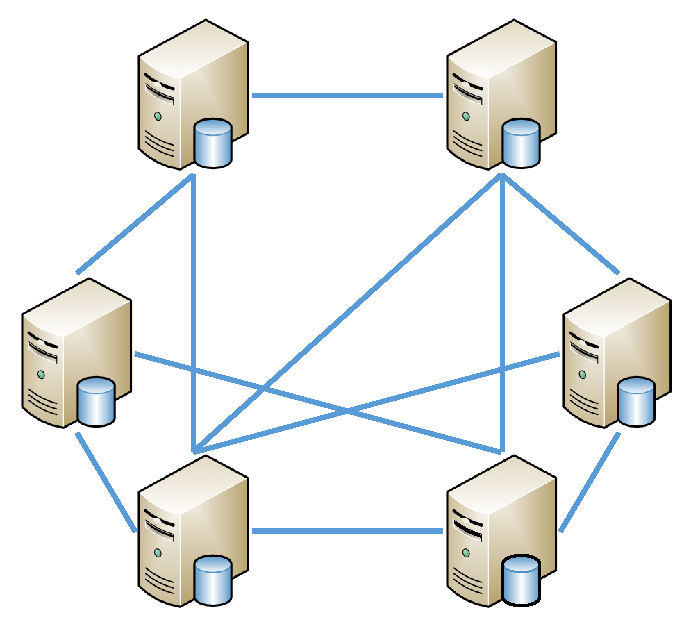
\includegraphics[width=1.78in]{Fig/chapter1/p2p.eps}
         	}
         	\subfigure[主从式]{
         		\label{fig:MS}
         		
         		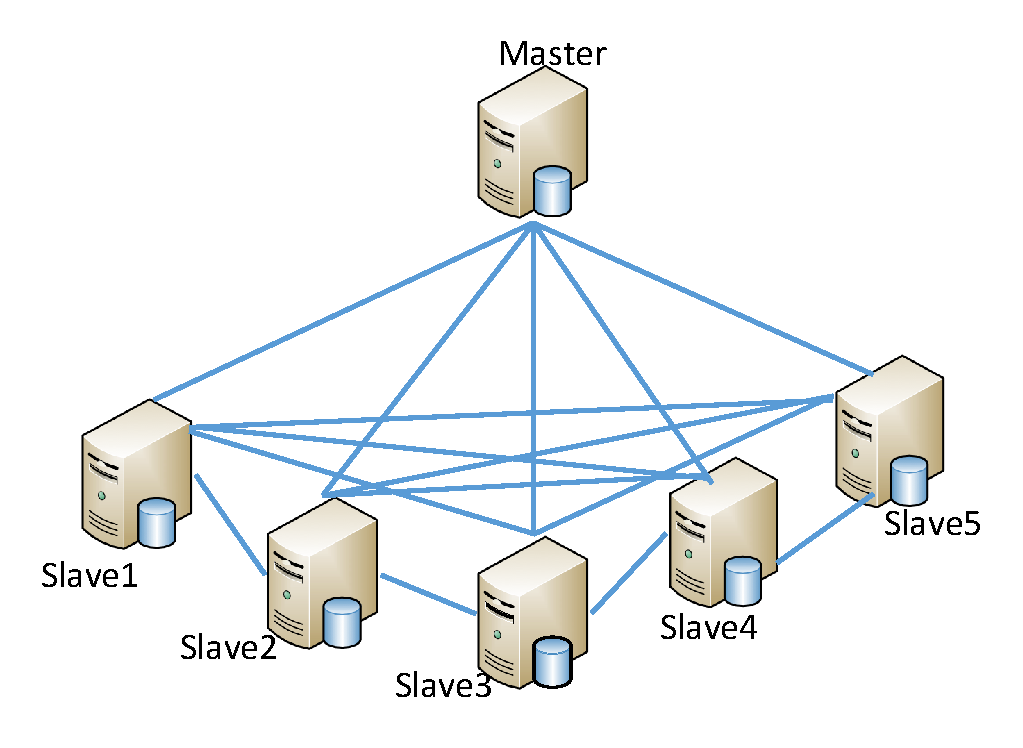
\includegraphics[width=1.78in]{Fig/chapter1/MasterSlave.eps}
         	}
         	\subfigure[协调者-远程结点式]{
         		\label{fig:CR}
         		
         		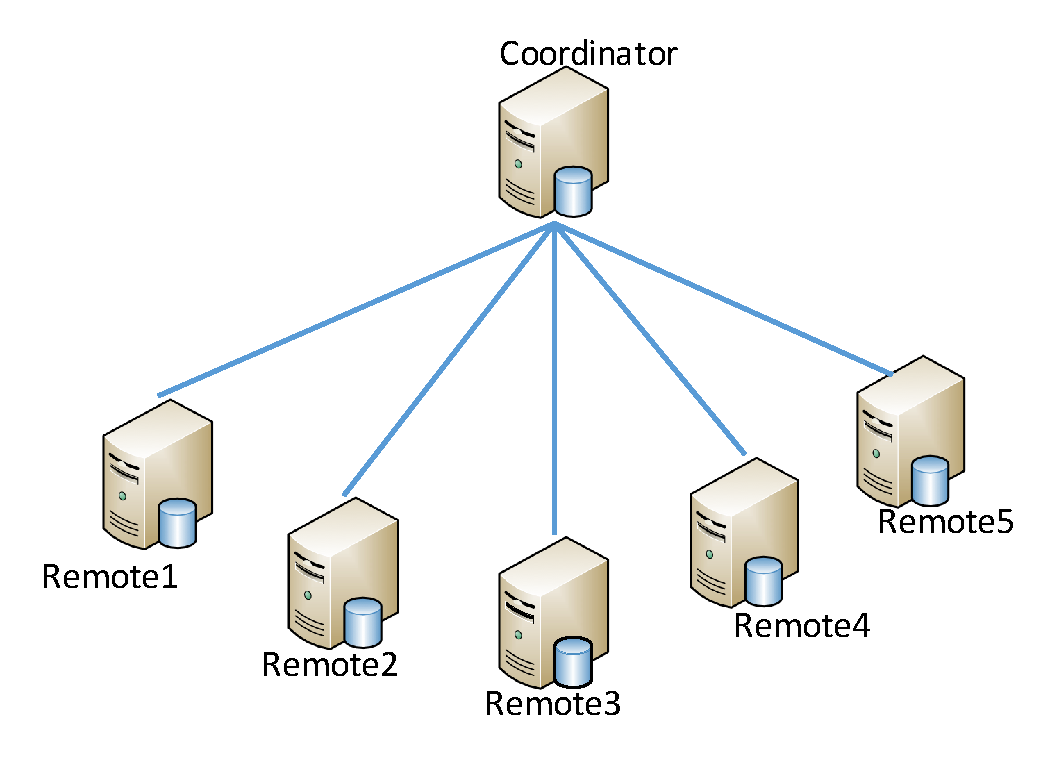
\includegraphics[width=1.78in]{Fig/chapter1/CoorRemote.eps}
         	}
         	\caption{3种常见分布式架构}
         	\label{fig:DistributeArc}
         \end{figure}
         
         此外,轨迹数据由于来源广、数据量大等特性,往往以分布式形式采集和存储在各结点中。这类结点既可以是管理着大量轨迹数据的高性能服务器也可以是管理单一移动对象的的个人智能手机。此外,结点间可能相互独立,不能互相访问。因此,
         如何对分布在具有不同存储和计算能力的各个结点上的分布式轨迹数据进行统一的管理、分析和挖掘服务是合理利用迹数据的首要问题。现有的分布式解决方案可分为以下三类:(i)基于对等系统(Peer-To-Peer,P2P)架构的处理方案。该架构中各个结点能互相访问且各个结点都有原始数据的完整备份,因此不适用与轨迹大数据。
         (ii)基于主-从式(Master-Slave)的分布式集群架构的处理方案。该架构中由一个主(Master)结点和多个从(Slave)结点构成,其中从结点存放具体数据并负责任务的执行,主结点存放数据的元数据并负责任务的分发和调度。基于该类架构典型的处理系统有Hadoop和Spark。该架构往往要求所有物理结点在同一个集群内部,结点间通过高速网络连通。
         (iii)基于协调者-远程结点的(Coordinator-Remote Site)的分布式架构。该架构中存在一个协调者和多个远程节点,其中协调者结点不存储任何数据只负责跟远程结点通信,而远程结点负责存放本地数据,且各远程结点间互不通信。 
         第三种方案可看做第二种方案的推广,首先它允许所有结点物理上互相远离,不要求它们位于同一集群内部。其次,远程结点间做到完全独立且互不知晓。最后,协调者结点不需要知道远程结点数据的任何信息。
         以上三点能有效地保证数据拥有者的隐私和数据存储、计算的独立性。因而,本文研究的分布式场景选择第三种处理框架。
   %      第一种架构要求数据共享,这不符合目前轨迹数据源间相互独立互不共享的特性。第二种架构要求数据集中在同一个物理集群中,而现实的轨迹数据存放在物理上相互远离互不知晓的节点中。第三种架构中,协调者节点用于接受用户的查询请求,各远程节点各自保存本地数据且互不知晓,远程节点仅与调节着结点进行通信。
  %    因此,前两个架构均不符合轨迹大数据的实际存储状况,仅第三种架构符合我们的需求。  
  
  目前,分布式轨迹相似度研究已经得到广泛的重视。文献\cite{setSimilar,kimICDE2012}研究了主-从式架构下轨迹数据的join查询,其关注重点是如何降低从节点间数据交换量过高的问题。文献\cite{CIKMSimilarity} 研究了基于协调者-远程节点架构下的$k$近邻轨迹查询研究。其研究的是用户手机连接基站的轨迹数据并将每个基站看作一个远程节点。由于手机在用户移动过程中会连接到不同的基站,故轨迹数据被切割成若干数据片段存放在不同的基站中。在该研究中,其研究目标是如何提高查询的效率而未关注如何降低通信开销。类似的,
Smart Trace\cite{SmartTrace} 和 Smart Trace$^{+}$ \cite{crowdsourced} 在相同的系统架构中研究了相同的问题,但在其研究内容中,将每个智能手机看做远程结点且每个结点仅保存一条轨迹数据。在这两项工作中,计算效率和通信开销同时得到了考虑。与以上不同的是,本文研究了更加通用的分布式场景,即每条轨迹完整的保存在一台远程结点上,且每个远程结点存储多条轨迹数据。
此外,文献\cite{trajectoryVLDB}提出了基于Spark的$k$近邻轨迹查询系统。该系统由于不满足应用中远程结点间相互独立、互不知晓的要求,因而无法推广到本文所提查询中。
  
  		                                                                                              

\section{研究内容与挑战}\label{sec-c1-content}
\begin{figure}
	\centering
	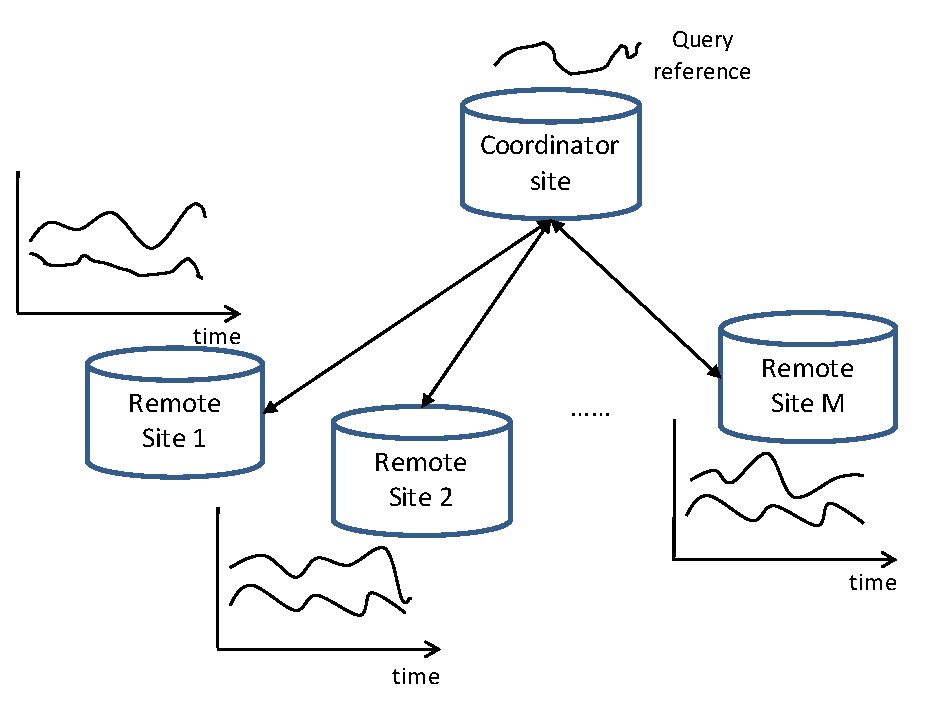
\includegraphics[width=0.73\textwidth]{Fig/chapter1/coor-remote}
	\caption{基于协调者-远程结点架构的查询展示}
	\label{fig-chapter1-demonstrate}
\end{figure}

本文选用基于协调者-远程节点的分布式架构进行管理和分析轨迹大数据,并对轨迹大数据上的$k$近邻轨迹查询进行了研究。该系统架构中存在一个协调者结点和$M$个远程结点。协调者节点和所有远程结点连通,但不知道远程结点上数据的任何信息。远程结点间彼此独立且互不通信。在实现查询过程中,协调者结点扮演查询引擎的角色,其接受用户提交的查询,并将查询相关数据发送给远程结点。每个远程结点根据接收到的数据返回相应的查询结果。
综上所述,本文所研究的查询如图\ref{fig-chapter1-demonstrate}所示。协调者节点负责接收用户提交的查询轨迹,每个远程结点存储一部分轨迹数据。协调者节点的目标是从所有远程结点中找出与查询对象最相似的$k$条轨迹。
一个直观的解决方案就是用户将$\cal Q$提交给协调者结点后,该结点直接将$\cal Q$发送给所有的远程结点。远程结点接收到查询对象后,计算其与本地存储的所有轨迹间的距离并将相似度值返回给协调者结点。最终,协调者结点从接收到的距离值中选择最小的$k$个作为结果返回给用户。这样的解决方案,设计简单且易于实现。但也存在着通信量过大的问题,尤其是当待查询轨迹数据量较大或远程结点较多时。因此,如何降低通信开销是我们需要解决的首要问题。此外,该方案中由于需要对查询轨迹和远程结点间的轨迹进行距离值计算,而距离计算往往耗时较多从而导致该方案计算开销也较大。为此,我们还需要考虑如何提高查询的执行效率。
最后,如上节所介绍,轨迹间的距离计算准则很多,现有工作只针对某一具体距离来进行通信或效率优化。因而,缺乏统一的框架或方法来处理。综上所述,
本文研究面临的挑战主要表现为以下3点:
\begin{itemize}
	\item  \textbf{首先,针对时间序列上已有的$k$近邻轨迹查询技术往往只针对某一距离准则设计,缺乏通用性。}距离度量选择准则是轨迹数据挖掘分析的核心内容之一,选用不同的度量函数,导致的挖掘结果以及对结果的理解往往大不相同。现有的工作都是针对某一研究问题,精心挑选或自定义一距离函数以满足研究的需要。因此,所提出的解决方案具有较高的局限性,很难推广到其他的问题中。为此,需要提出通用或对一类问题适用的解决方案。
	
	\item \textbf{其次,现有分布式$k$近邻查询算法中仍然存在着通信开销过大的问题。}直接将原始查询轨迹发送到所有远程结点的方式,其通信开销随轨迹长度和远程结点的个数的增加而快速增大。而现有的数据降维方案如Douglas-Peuker算法、奇异值分解(Singular Value Decomposition, SVD)、离散傅里叶变换(Discrete Fourier Transform, DFT)、哈尔小波变换(Haaar Wavelet Transform, HWT)、分段聚合近似(Piecewise Aggregate Approximation, PAA)、自适应分段常量近似(Adaptive Piecewise Constant Approximation, APCA)等方法虽然降低了数据的维度,但也造成了数据信息损失,使得数据不再直观且不能保证结果的准确性。此外,这些方法常用于处理一维时间序列数据,而轨迹是天然的多维时间序列数据。为此,需要提出新的轨迹数据降维方法,在保证查询结果正确性的同时,降低通信开销。

	\item \textbf{最后,现有的分布式top-$k$查询时间效率需要得到提升。}轨迹距离的计算除欧式距离是一次的计算复杂度,其他往往需要二次的计算复杂度。在每个远程结点进行查询轨迹与局部保存的轨迹进行两两相似度计算的方案不可行。虽然适用传统索引技术是加快查询速度有效工具,但索引技术只能针对原始轨迹数据,无法适用于降维后的数据。为此,需要设计新的方案来提高查询效率。
	
\end{itemize}

\section{主要贡献}\label{sec-c1-contribution}
本文围绕分布式$k$近邻轨迹查询这一问题,系统性的提出了解决方案。首先,针对轨迹距离度量的多样性,提出了两种查询实现框架以覆盖所有的距离函数。这两个框架分别针对不同类别的距离度量准则,在保证查询结果正确性的同时能有效地降低通信开销。接着,我们将两个常用轨迹距离函数分别嵌入到两个框架中,并提出了对应的算法。最后,使用真实轨迹数据集验证了算法的性能。因此,本文的主要贡献分为以下3点:
\begin{itemize}
	\item  \textbf{针对通信开销较高问题,提出了两个通用查询实现框架FTB(Framework with Two Bounds)和FLB(Framework with Lower Bound)。}FTB框架中要求能根据降维后的概要数据计算出相似度距离的上、下界,并且需保证当细粒度的概要数据获取后,所计算出来的上、下界越来越紧并最终能收敛。FLB框架中仅要求能根据降维后的概要数据计算出相似度距离的下界,且仅需保证当细粒度的概要数据获取后,所计算出来的下界越来越紧。这两个框架由于仅需要传递查询轨迹的概要数据且仅需计算复杂度更低的界信息,因此能大大降低通信和计算开销。
	
	\item \textbf{针对FTB框架,提出了基于欧式距离的FTB-ED 算法。}为验证FTB框架的有效性,本文研究了如何将欧式距离嵌入到该框架中。为此,本文首先利用Haar小波变换以得到不同粒度的轨迹概要数据,并证明了全部概要数据的欧式距离等于原始轨迹数据的欧式距离。接着,利用部分概要数据,本文提出了针对欧式距离的轨迹相距离上、下界,并理论证明了界函数的正确性。然后,我们将该上、下界应用到FTB框架中,提出了FTB-ED算法。在该算法中,我们引入了性能优化策略以提高查询效率。
	最后,我们通过理论分析和大量实验验证了FTB-ED算法的有效性和可扩展性。
	
	\item  \textbf{针对FLB框架,提出了基于动态时间卷曲距离的FLB-DTW算法。}为验证FLB框架的有效性,本文研究了如何将动态时间卷曲距离嵌入到该框架中。
	为此,本文首先针对查询轨迹使用不同粒度的包围信封(Bounding Envelope)来表示轨迹的概要数据。接着提出了基于动态时间卷曲距离的下界,并理论证明了该下界的正确性。最后将该下界应用到FLB-DTW框架中,并提出了FLB-DTW算法。在该算法中我们引入了索引等多种机制以提高查询效率。最后,我们通过大量实验验证了FLB-DTW算法的有效性和可扩展性。
	
\end{itemize}


\section{章节安排}
\begin{figure}
	\centering
	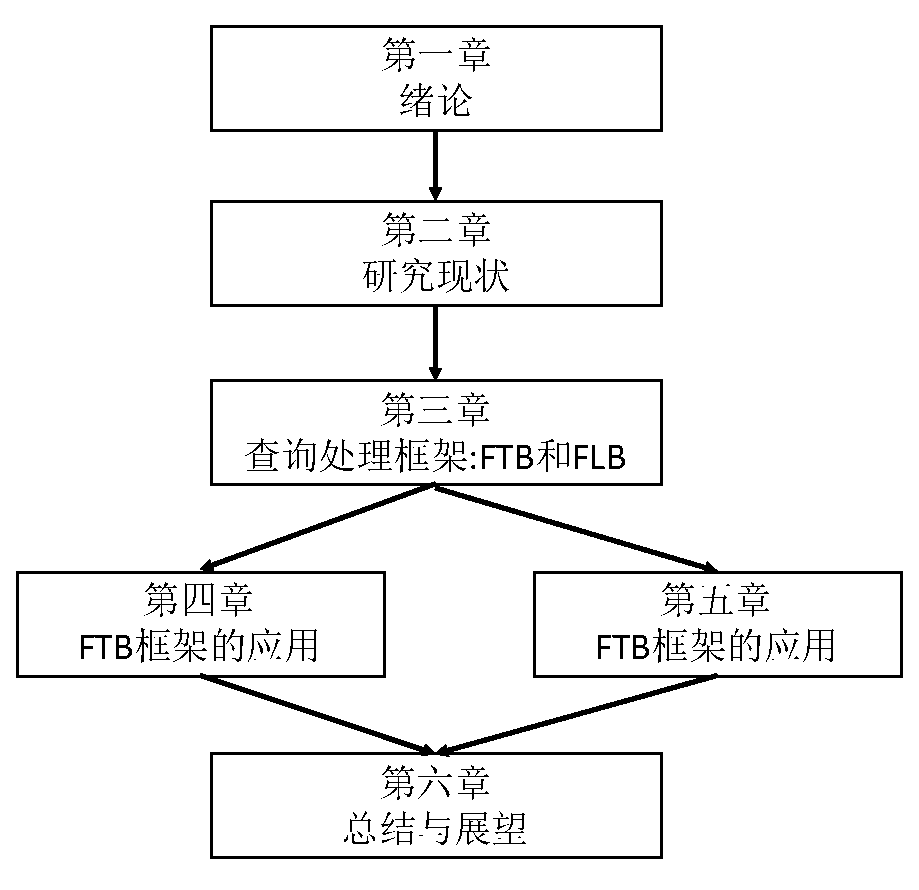
\includegraphics[width=0.63\textwidth]{Fig/chapter1/paperStructure}
	\caption{本文的组织结构}
	\label{fig-chapter1-structure}
\end{figure}
本文一共分为六章,章节安排如图~\ref{fig-chapter1-structure}所示:
\begin{itemize}
	\item 第二章从轨迹数据存储、轨迹降维以及轨迹数据相似性查询三个方面介绍了研究背景知识和研究现状。
	\item 第三章介绍了两个通用查询处理框架FTB和FLB以分别处理能同时提供上、下界的和仅能提供下界的距离准则函数。
	\item 第四章介绍了如何将欧式距离嵌入到FTB框架中,并提供高效的查询结果。
	\item 第五章介绍了如何将动态时间卷曲距离嵌入到FLB框架中,并提供高效的查询结果。
	\item 第六章对上述已有工作进行了总结,并展望了未来的研究方向和内容。
\end{itemize}

\clearpage
\phantom{s}
\clearpage